\documentclass[tikz,border=5mm]{standalone}
\usepackage{tikz}
\usetikzlibrary{arrows.meta}
\usepackage{amsmath}
\usepackage{physics}

\ExplSyntaxOn
\msg_redirect_name:nnn { siunitx } { physics-pkg } { none }
\ExplSyntaxOff

\begin{document}
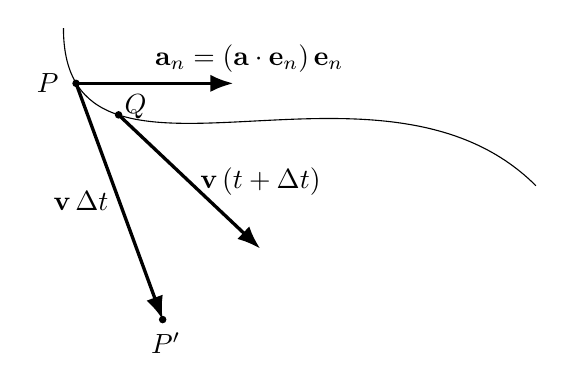
\begin{tikzpicture}[scale=2,
		vector/.style={-{Latex}, very thick}]

    \draw (0, 0.5) .. controls (0, -0.75) and (2, 0.5) ..  (3, -0.5);
    
    \node at (-0.1, 0.15) {$P$};
    \node at (0.458, 0) {$Q$};
    \node at (0.65, -1.5) {$P^{\prime}$};


    \draw [fill] (0.08, 0.15) circle (0.02);
    \draw [fill] (0.35, -0.05) circle (0.02);
    \draw [fill] (0.63, -1.35) circle (0.02);

    \draw [vector] (0.08, 0.15) -- ++(1, 0) node [pos=1.1, above] {$\vb{a}_{n} = \left( \vb{a} \cdot \vb{e}_{n} \right) \vb{e}_{n}$};
    
    \draw [vector] (0.08, 0.15) -- ++(0.55, -1.5) node [midway, left] {$\vb{v} \, \Delta t$};
    \draw [vector] (0.35, -0.05) -- ++(0.9, -0.85) node [midway, right] {$\vb{v} \left( t + \Delta t \right)$};

\end{tikzpicture}
\end{document}